\documentclass{article}

\usepackage[hidelinks]{hyperref}
\usepackage{graphicx}
\usepackage{titling}
\usepackage{float}
\usepackage[text={18cm,21cm},centering]{geometry}
\usepackage{enumitem}
\hypersetup{
	colorlinks=true,
	linkcolor=blue,
	urlcolor=blue
}

\begin{document}
	
	\begin{titlepage}
		\centering
		{\bfseries\LARGE Universidad de La Habana \par}
		\vspace{1cm}
		{\scshape\Large Facultad de Matemática y Computación \par}
		\vspace{3cm}
		{\scshape\Huge Primer Proyecto de Simulación \par}
		\vfill
		
		{\Large Ana Paula González Muñoz C-312 \par}
		{\Large Dennis Daniel González Durán C-312 \par}
		{\Large Frank H. Perez Fleitas C-312 \par}
		\vfill
		{\href{https://github.com/anamunnoz/Simulation-Project}{Proyecto en github} \par}
	\end{titlepage}


	\section*{Introducción}
	Este proyecto tiene como objetivo desarrollar una simulación de eventos discretos para entender mejor el problema orientado. Se busca aplicar los principios de la simulación de eventos discretos para modelar y experimentar con estos fenómenos, y obtener resultados que nos ayuden a tomar decisiones informadas.
	
	\subsection*{Objetivos y metas}
	\begin{enumerate}
		\item  Desarrollar un sistema que permita modelar el problema
		\item Utilizar el sistema para basándonos en sus resultados y en el análisis estádistico de estos, tomar decisiones.
		\end{enumerate}
	
	\subsection*{Sistema específico a simular: Central Telefónica}
	
	La compañía aérea “Siberia” tiene una centralita de teléfonos con 3 líneas. La empresa tiene un pico de llamadas durante 3 horas, en las que algunos clientes no pueden ponerse en contacto con la empresa debido al intenso tráfico de llamadas (se sabe que si las tres líneas están siendo utilizadas al cliente no se le puede retener). La compañía estima que, debido a la fuerte competencia, el 60\% de las	llamadas no respondidas utiliza otra compañía. Durante las horas punta las llamadas siguen una distribución de Poisson con una media de 20 llamadas hora, mientras que en el resto del tiempo la media es de 5 llamadas hora. Cada telefonista emplea 6 minutos por cada llamada (distribución exponencial). El beneficio de un viaje distribuye normal con una media de  210 euros y varianza de 50. Cada empleado cuesta a la compañía 24 euros/hora y una linea telefonica debe ser atendida por uno de ellos. Se asume que el coste de añadir una línea es despreciable.
	
	\begin{itemize}
		
		\item Parámetros del sistema:
		\begin{itemize}[left=2em]
			\item Media de llamadas en horas no punta
			\item Media de llamadas en horas punta
			\item Media del tiempo de atención de una llamada
			\item Duración de la simulacóon
			\item Cantidad de líneas operando
			\item Intervalos de horas punta
			\item Media del costo de un viaje
			\item Varianza del costo de un viaje
			\item Valor de probabilidad de que los clientes usen otra compañía
		\end{itemize}
		
		\item Variables de interés:
		\begin{itemize}[left=2em]
			\item Llamadas atendidas
			\item Llamadas perdidas
			\item Ganancia por llamadas atendidas
			\item Cantidad de clientes que usaron otra compañía
		\end{itemize}
	\end{itemize}
	
	\section*{Detalles de implementación}
	En el directorio source se encuentra el archivo que contienen el código fuente de la simulación. El mismo se divide en diferentes secciones:
	
	\subsection*{Métodos y estructuras auxiliares}
	Se definen métodos de utilidad para la simulación:
	\begin{itemize}[left=2em]
		\item \textbf{make\_central:} crea una central telefónica con la cantidad de líneas especificada. La central se comporta como un arreglo de booleanos, donde en la i-ésima posición se almacena si dicha línea está ocupada o no.
		\item \textbf{calculate\_salaries:} dado una cantidad de líneas y un salario por horas determina cuanto dinero pierde la central como pago a los trabajadores.
		\item \textbf{stop\_case:} determina si la simulación debe detenerse. Para esto realiza un análisis por intervalos de confianza para comprobar si se tiene suficiente información de las variables objetivos.
		\item \textbf{mean\_call:} determina en un momento de la simulación la media de la distribución con la que llegan llamadas a la central en dependencia de las horas puntas
	\end{itemize}
	
	Se definen estructuras de utilidad para la simulación:
	\begin{itemize}[left=2em]
		\item \textbf{class Config:}  entidad donde se almacenan los parámetros de la simulación
		\item \textbf{class Event:} representación de un evento. Estos tienen tipo, tiempo restante para que ocurra y posición en la central en caso de ser una llamada que está siendo atendida
	\end{itemize}
	
	\subsection*{Simulación del problema}
	Se encuentra el código principal de la simulación que funciona con una cola de eventos de la siguiente manera:
	\begin{itemize}[left=2em]
		\item Se crea una central telefónica 
		\item Se genera la primera llamada entrante y se inserta en la cola 
		\item Mientras no se cumpla el caso de parada se simula un día en la central. Para esto se toma el evento de la cola más próximo a ocurrir 
		\begin{itemize}
			\item En caso de ser una llamada: se inserta en la cola y se generan dos nuevos eventos: la finalización de esta y la entrada de una nueva llamada.
			\item En caso de ser la finalización de una llamada: se libera la línea telefónica que esta utiliza
		\end{itemize}
		Al finalizar el día, se almacena el resultado de las variables de interés y se comprueba el caso de parada para determinar si es necesario que la simulación continue.
	\end{itemize}
	
	\subsection*{Análisis estadístico}
	Se encuentran los códigos correspondientes a las gráficas y pruebas de hipótesis que se muestran en el informe.

	
	\section*{Resultados y experimentos}
		El modelo tiene la forma:
		\begin{itemize}[left=2em]
			\item Media de llamadas en horas no punta = 5
			\item Media de llamadas en horas punta = 20
			\item Media del tiempo de atención de una llamada = 6
			\item Cantidad de líneas operando = 3
			\item Intervalos de horas punta = [[3,6]]
			\item Media del costo de un viaje= 210
			\item Varianza del costo de un viaje= 50
			\item Valor de probabilidad de que los clientes usen otra compañía= 0.6
	   \end{itemize}
	
		Durante la simulación la central telefónica generó una ganancia promedio de 29714 euros por día. En promedio, se dejaron de atender 13 llamadas diarias, resultando en una pérdida potencial de 7 clientes por día debido a las llamadas no atendidas.
		
		Los resultados indican que, aunque la ganancia promedio diaria es significativa, la pérdida debido a las llamadas no atendidas podría representar una oportunidad de mejora. Reducir el número de llamadas no atendidas podría aumentar considerablemente la ganancia total.
		
		\subsection*{Formulación de hipótesis de la simulación}
			En esta sección se presentan las hipótesis que guiarán la simulación de la central telefónica, con el objetivo de evaluar su impacto en la ganancia generada. Se plantean dos hipótesis principales:
			
			\subsubsection*{Hipótesis 1: Incremento en la cantidad de líneas telefónicas}
			
			\textbf{Descripción:} Se propone que aumentar el número de líneas telefónicas en la central reducirá la cantidad de llamadas perdidas y aumentará la cantidad de llamadas atendidas, lo que podría incrementar la ganancia.
			
			Para comprobar esto se realizó una simulación para cada cantidad de líneas (entre 0 y 8) para promediar la ganancia (teniendo en cuenta el salario de los trabajadores). Se muestran los resultados en la siguiente gráfica:
			
				\begin{figure}[H]
				\centering
				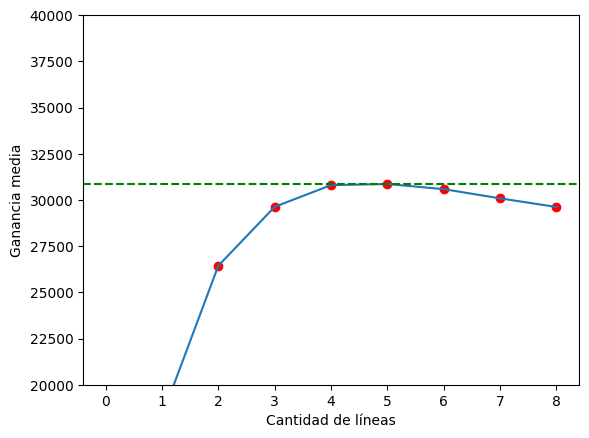
\includegraphics[width=0.7\linewidth]{./output.png}
				\label{fig:enter-label}
			\end{figure}
			
			Se puede observar que en promedio se obtiene mejor ganancia con 4, 5 y 6 líneas.
			
			Para apoyar esta idea, se observó también la cantidad de llamadas perdidas según la cantidad de líneas telefónicas activas:
			
			\begin{figure}[H]
				\centering
				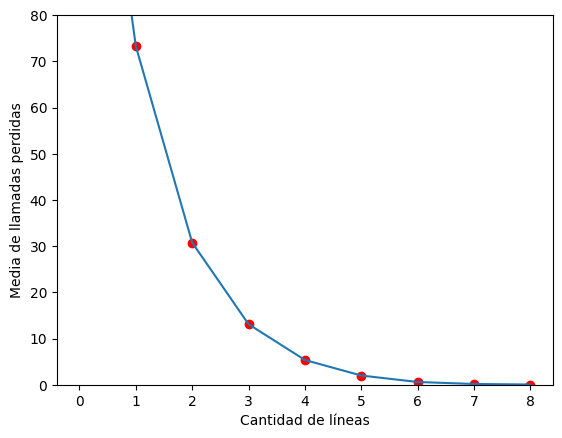
\includegraphics[width=0.7\linewidth]{./output1.png}
				\label{fig:enter-label}
			\end{figure}
			
			Se puede observar que de 4 líneas en adelante se pierden menos llamadas, por lo que se puede suponer que con 5 líneas se atienden la mayor cantidad de llamadas y por lo tanto se obtiene una mayor ganancia en promedio.
			
			\vspace*{0.5cm}
			Se realiza una prueba de hipotésis para comprobar si las diferencias entre las ganancias con 3 y 5 líneas son significativas o no: \\
			$H_o: \mu_1 = \mu_2 $\\
			$H_a: \mu_i \neq \mu_j$ \\
			
			Cuando se analiza el intervalo de confianza con $\alpha=0.05$ de la diferencia entre ambos sistemas obtenemos un $p-value = 2.2287551656043974e-116$ por lo que se rechaza la hipótesis nula: la central obtiene mayor ganancia con 5 trabajadores que con 3.
			
			\vspace*{0.5cm}
			Se realiza una segunda prueba de hipotésis para comprobar si las diferencias entre las llamadas perdidas con 3 líneas y con 5 son significativas o no: \\
			$H_o: \mu_1 = \mu_2 $\\
			$H_a: \mu_i \neq \mu_j$ \\
			
			Cuando se analiza el intervalo de confianza con $\alpha=0.05$ de la diferencia entre ambos sistemas obtenemos un $p-value = 0$ por lo que se rechaza la hipótesis nula: la central pierde menos llamadas 5 trabajadores que con 3.
			
			
			\subsubsection*{Hipótesis 2: Reducción del tiempo de atención}
			
			\textbf{Descripción:} Se plantea que disminuir el tiempo promedio de atención por llamada permitirá gestionar un mayor número de llamadas en el mismo período, optimizando el rendimiento de la central y aumentando las ganancias.
			\smallskip
				
			Para comprobar esto se realizó una simulación para cada tiempo de demora de atención de las llamadas (entre 0 y 6 minutos por llamada) y la cantidad de líneas del modelo original (3) y variando el tiempo de atención (entre 0 y 6 minutos por llamada). Se muestran los resultados en la siguiente gráfica:
			
			\begin{figure}[H]
				\centering
				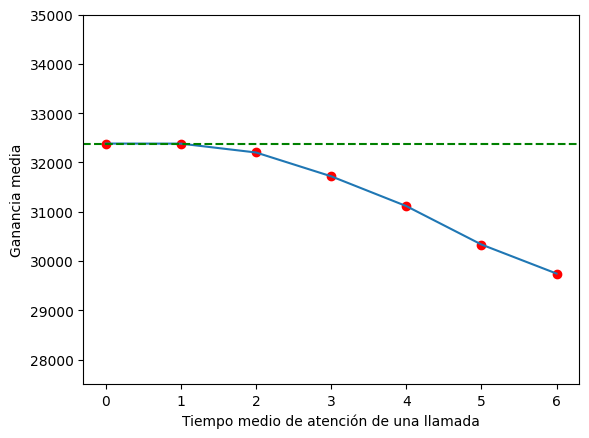
\includegraphics[width=0.7\linewidth]{./output3.png}
				\label{fig:enter-label}
			\end{figure}
			
			Se puede observar que en a medida que disminuye el tiempo de atención se obtiene mayor ganancia.
			
			Para apoyar esta idea, se observó también la cantidad de llamadas perdidas según el tiempo de atención:
			
			\begin{figure}[H]
				\centering
				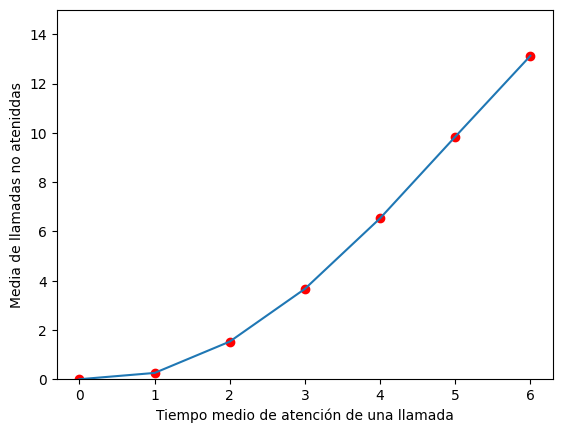
\includegraphics[width=0.7\linewidth]{./output2.png}
				\label{fig:enter-label}
			\end{figure}
			
			Se puede observar que a medida que disminuye el tiempo de atención disminuye la cantidad de llamadas perdidas. 
			\smallskip
			
			\subsection*{Comparación entre las hipótesis de la simulación}
			Para decidir cuál estrategia es mejor para optimizar la ganancia de la central se compararán los resultados obtenidos en ambas. 
			\vspace{0.2cm}
			
			Como se puede observar en la siguiente gráfica, para superar las ganancias generadas por 5 líneas telefónicas se necesita que el tiempo de atención tenga una media menor que 4 minutos por llamada. 
			
			\begin{figure}[H]
				\centering
				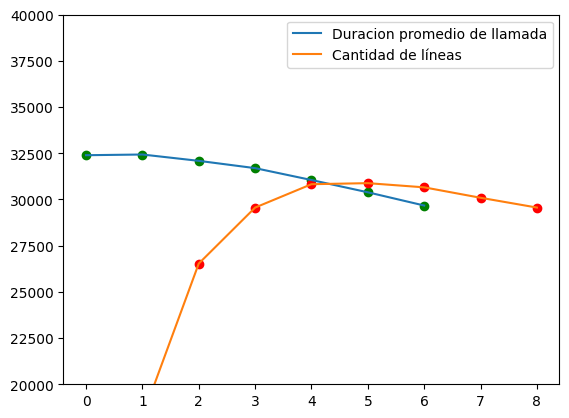
\includegraphics[width=0.7\linewidth]{./output5.png}
				\label{fig:enter-label}
			\end{figure}
			
			Los resultados sugieren que si el deseo de la empresa es aumentar las ganancias se tienen dos opciones principales:
			
			\begin{itemize}[left=3em]
				\item Aumentar a 5 la cantidad de líneas telefónicas.
				\item Disminuir a 4 minutos o menos la media del tiempo de atención por llamada.
			\end{itemize}
			
			
			La elección de alguna de estas estrategias depende del costo y viabilidad de disminuir el tiempo de atención.
			\vspace{0.4cm}
			
			Además si la empresa desea lograr una mayor satisfacción de los clientes se podría analizar la perdida de llamdas según cada estrategia.
			
			
			\begin{figure}[H]
				\centering
				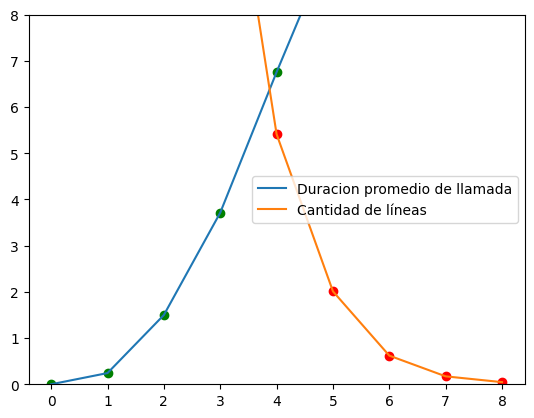
\includegraphics[width=0.7\linewidth]{./output4.png}
				\label{fig:enter-label}
			\end{figure}
			
			Se realiza una prueba de hipotésis para comprobar si las diferencias entre las llamadas no atendidas con 5 líneas es significativa  con respecto a las llamadas perdidas con una media de atención de 4 minutos: \\
			$H_o: \mu_1 = \mu_2 $\\
			$H_a: \mu_i \neq \mu_j$ \\
			
			Cuando se analiza el intervalo de confianza con $\alpha=0.05$ de la diferencia entre ambos sistemas obtenemos un $p-value = 0$ por lo que se rechaza la hipótesis nula: las diferencias entre las llamadas no atendidas de ambas estrategias es significativa.
			\vspace{0.3cm}
			
			Se puede observar entonces que para obtener un valor cercano o mejor a la perdida de llamadas obtenidas con 5 líneas telefónicas se necesita al menos una media de atención de 3 minutos por llamada, por lo que si se tiene en cuenta la satisfacción de los clientes se necesitará disminuir a 3 minutos o menos la media del tiempo de atención, por lo que será decisión de la empresa que estrategia aplicar según la viabilidad y el presupuesto disponible.
			
			\subsection*{Análisis de parada de la simulación}
			La simulación se detiene por alguno de los siguientes 2 motivos:
			\begin{itemize}[left=3em]
				\item Se alcanza la cantidad máxima de días de la simulación
				\item Se cumple el caso de parada definido en \textbf{stop\_case}
				\begin{itemize}
					\item Se utiliza un intervalo de confianza $\alpha$ = 0.05 y por lo tanto Z{$\alpha$}/2 = 1.96. Esto significa que será cierto, con una probabilidad (aproximadamente) igual a 0.95, que la media muestral X y la desviación estándar muestral S serán tales que la media poblacional estará entre $X \pm 1.96/\sqrt{n}$
				\end{itemize}
			\end{itemize}
			
			
		
\end{document}